\documentclass[a4paper,10pt,oneside]{jsbook}
%
\usepackage{amsmath,amssymb,bm}
\usepackage{bm}
\usepackage[dvipdfmx]{graphicx}
\usepackage{ascmac}
\usepackage{makeidx}
\usepackage{txfonts}
\usepackage{indentfirst}
\usepackage{booktabs}
\usepackage{tabularx}
\usepackage{comment}
\AtBeginDvi{\special {pdf:tounicode EUC-UCS2}}
\usepackage[dvipdfmx, setpagesize=false, bookmarks=true, bookmarksnumbered=true]{hyperref}
\usepackage{nameref}
\usepackage{url}
%
\makeindex
%
\newcommand{\diff}{\mathrm{d}}            %微分記号
\newcommand{\divergence}{\mathrm{div}\,}  %ダイバージェンス
\newcommand{\grad}{\mathrm{grad}\,}       %グラディエント
\newcommand{\rot}{\mathrm{rot}\,}         %ローテーション
%
\setlength{\textwidth}{\fullwidth}
\setlength{\textheight}{44\baselineskip}
\addtolength{\textheight}{\topskip}
\setlength{\voffset}{-0.6in}
%

\begin{document}

%%%%%%%%%%%%%%%%%%%%%%%%%%%%%%%%%%%%%%%%%%%%%%%%%%%%%
% 表紙
\begin{titlepage}
\noindent
独立行政法人 理化学研究所 御中
\begin{center}
	\vspace{8cm}
	{\Huge \textbf{協調ワークスペースドライバと}} \\
	\vspace{1cm}
	{\Huge \textbf{協調動作フレームワークのプロトタイプ}} \\
	\vspace{1cm}
	{\Huge \textbf{設計書}} \\
	\vspace{10cm}
	{\Large \textbf{2015年3月26日}} \\
	\vspace{0.5cm}
	{\Large \textbf{株式会社イマジカ デジタルスケープ}}
\end{center}
\end{titlepage}

%%%%%%%%%%%%%%%%%%%%%%%%%%%%%%%%%%%%%%%%%%%%%%%%%%%%%
% 目次
\tableofcontents

%%%%%%%%%%%%%%%%%%%%%%%%%%%%%%%%%%%%%%%%%%%%%%%%%%%%%
% 本文
%%%%%%%%%%%%%%%%%%%%%%%%%%%%%%%%%%%%%%%%%%%%%%%%%%%%%
\chapter{はじめに}
本書では協調ワークスペースドライバと協調動作フレームワークのプロトタイプの設計について解説します.

\chapter{システム構成について}
\section{全体の構成}
本システムは, node.js及びwebsocketsを用いたクライアントサーバプログラムであり, 複数のアプリケーションや,複数のユーザが共同作業を行える, 巨大なスクリーンスペースを, 仮想ディスプレイとして提供する. 構成図を図\ref{fig:system}に示す.

\begin{figure}[htbp]
	\begin{center}
		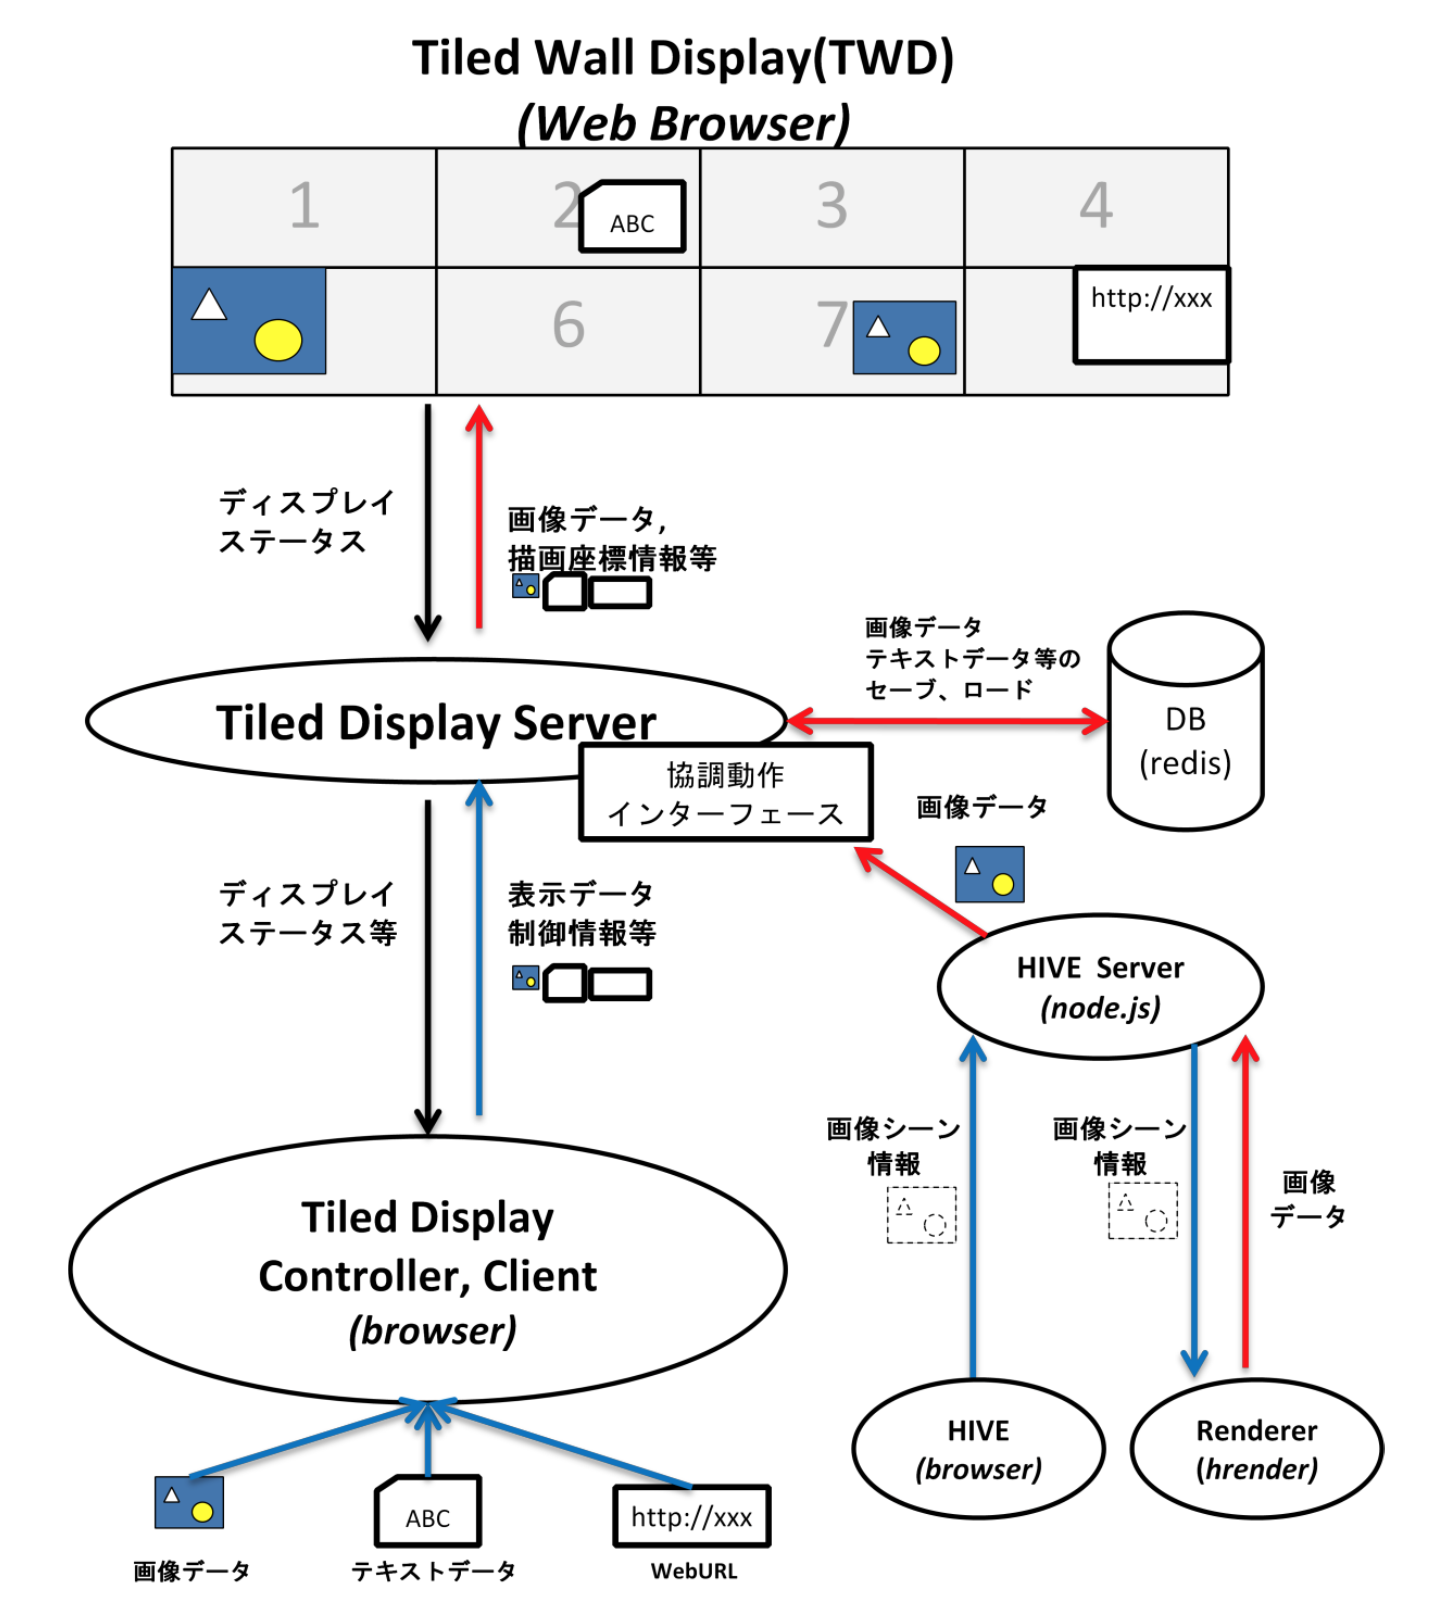
\includegraphics[width=11.5cm]{image/system.png}
	\end{center}
	\caption{構成図}
	\label{fig:system}
\end{figure}

\section{サーバとクライアントの役割}

\subsection{サーバの役割}
\begin{itemize}
\item HTTP通信 - クライアントに対してHTMLページなどを送信する
\item Socket.IO通信 - node.jsによる通信機能で, クライアントのコントローラとの間で通信を行う.
\item Websocket通信 - websocketプロトコルにより, クライアントのコントローラ及びディスプレイとの間で通信を行う
\item データベース入出力 - クライアントから送信された画像データやテキストデータをredisに保存し, 永続化する.
\item サーバサイドレンダリング - 送信されたURLのウェブサイトをphantomjsを用いてサーバサイドでレンダリングし, png画像として保存する.
\end{itemize}

\subsection{クライアント - コントローラの役割}
\begin{itemize}
\item ディスプレイの登録, 削除
\item ディスプレイの移動, 拡縮 などのメタデータ編集操作
\item コンテンツ(画像データ, テキスト, URL)の登録, 削除
\item コンテンツの移動, 拡縮 などのメタデータ編集操作
\item ディスプレイの分割数の設定
\item コンテンツデータのダウンロード
\end{itemize}

\subsection{クライアント - ディスプレイの役割}
\begin{itemize}
\item 自身のウィンドウをディスプレイとしてサーバへ登録
\item コントローラで設定されたとおりにコンテンツを表示.
\end{itemize}

\section{サーバの構成}

\subsection{サーバ}
サーバは, node.jsを使用して, socket.io及びwebsocketによる通信に対応している. それぞれの通信方法によって受付ポートを分けている. 

\begin{table}[htbp]
\begin{center}
\caption{受付ポート一覧}
\label{ports}
\begin{tabular}{|l|l|l|l|}
\hline
受付ポート & 通信方式 & クライアント & HTTPアクセス時 \\
\hline
\hline
ポートA & socket.io & socket.ioを用いたコントローラによって使用される & スタートページが表示される \\
\hline
ポートB & websocket & websocketを用いたディスプレイによって使用される & - \\
\hline
ポートC & websocket & websocketを用いたコントローラによって使用される & - \\
\hline

\end{tabular}
\end{center}
\end{table}

ポートA, ポートB, 及びポートCは, 連番になっており, デフォルトではポートA: 8080, ポートB: 8081 ポートC: 8082となっている.
ポート番号は, 起動バッチファイル内のnodeコマンドの引数を記述することにより, 変更することができる.

\subsection{データベース}
データベースはredisを使用して高速なレスポンスを実現している. 
データの格納方法については, \ref{redisdb}章を参照.

\subsection{その他ソフトウェア}
ウェブページレンダリング用にPhantomJS, 及びphantom.jsのnpmラッパーであるphantomjsを使用している.
ウェブページレンダリングはサーバサイドレンダリングを行っている.

\subsection{クライアントの構成}
クライアントサイドは, 仮想ディスプレイに対してコンテンツの追加登録等の操作を行う「コントローラ」と, 表示のみを行う「ディスプレイ」から構成されている.

\subsection{コントローラ}
コントローラは, socket.ioを用いてサーバと通信を行っている. 
サーバとの通信用 API の仕様については, \ref{connectionapi}章を参照.
コントローラの画面イメージを図\ref{fig:display}に示す.

\begin{figure}[htbp]
	\begin{center}
		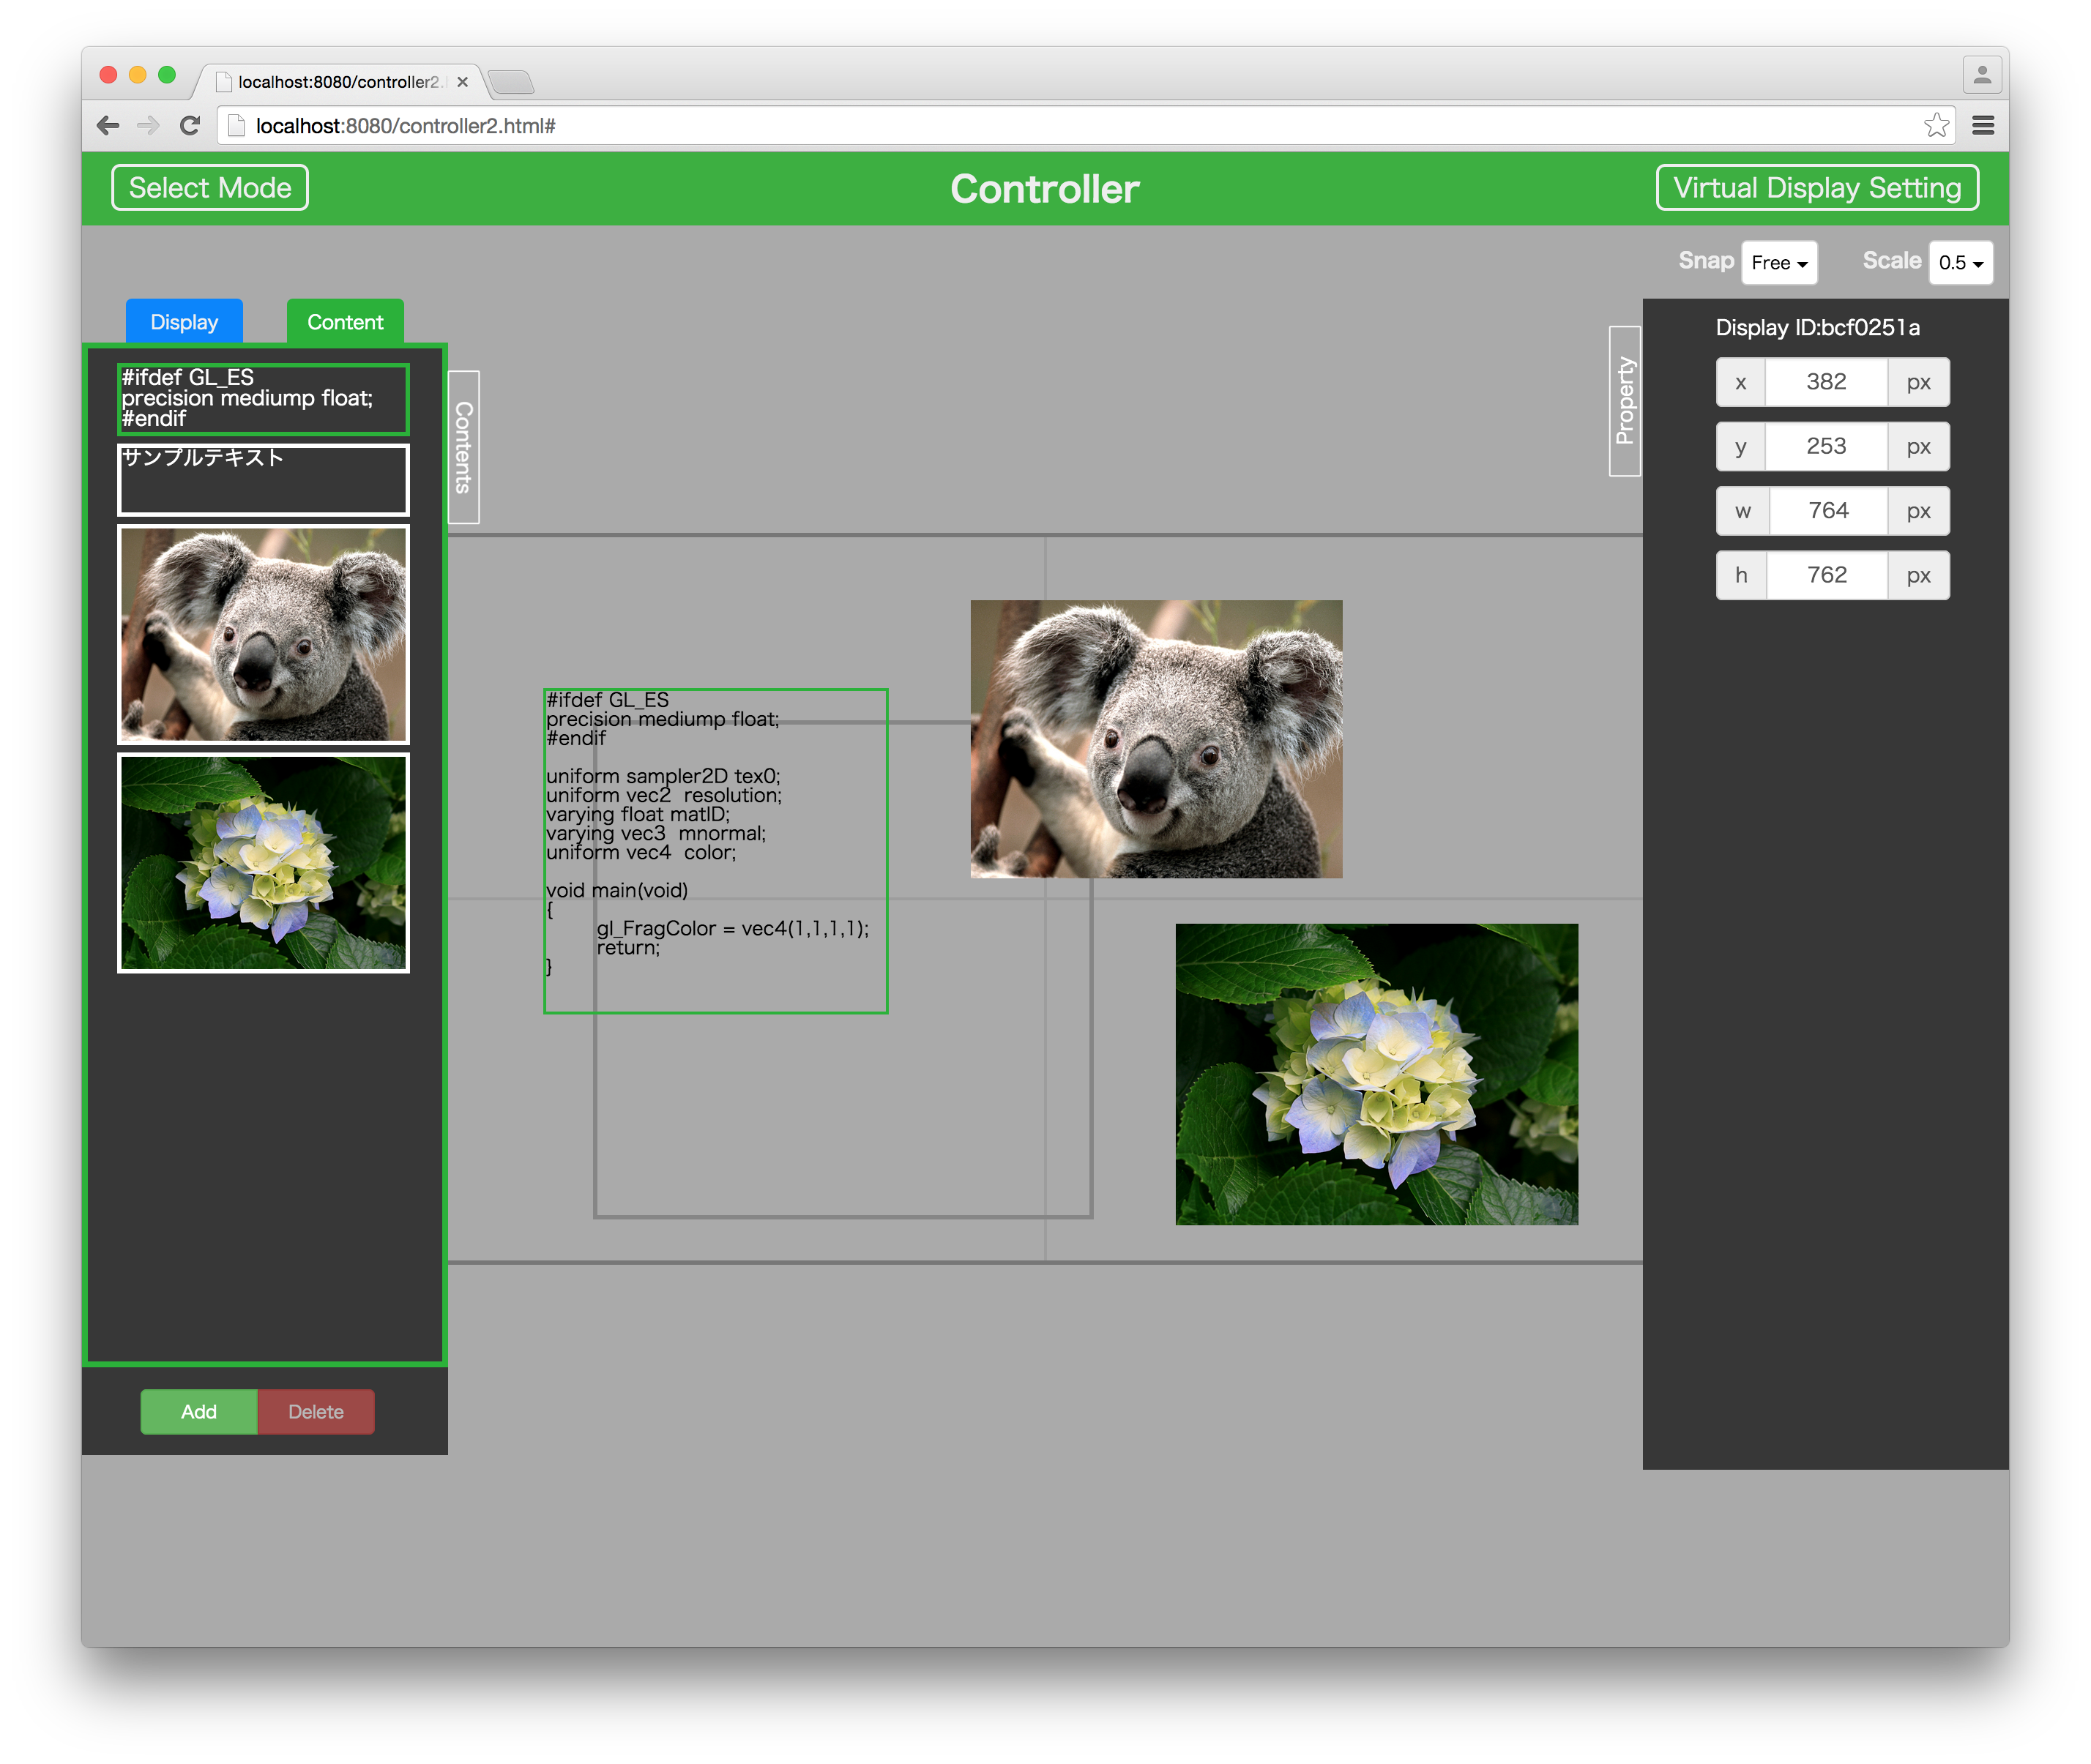
\includegraphics[width=14.5cm]{image/controller.png}
	\end{center}
	\caption{コントローラ画面}
	\label{fig:controller}
\end{figure}

\subsection{ディスプレイ}
ディスプレイは, コントローラで設定したコンテンツを表示する. HTML5の機能であるwebsocketを用いてサーバと通信している. ディスプレイのイメージを図\ref{fig:display}に示す. 

\begin{figure}[htbp]
	\begin{center}
		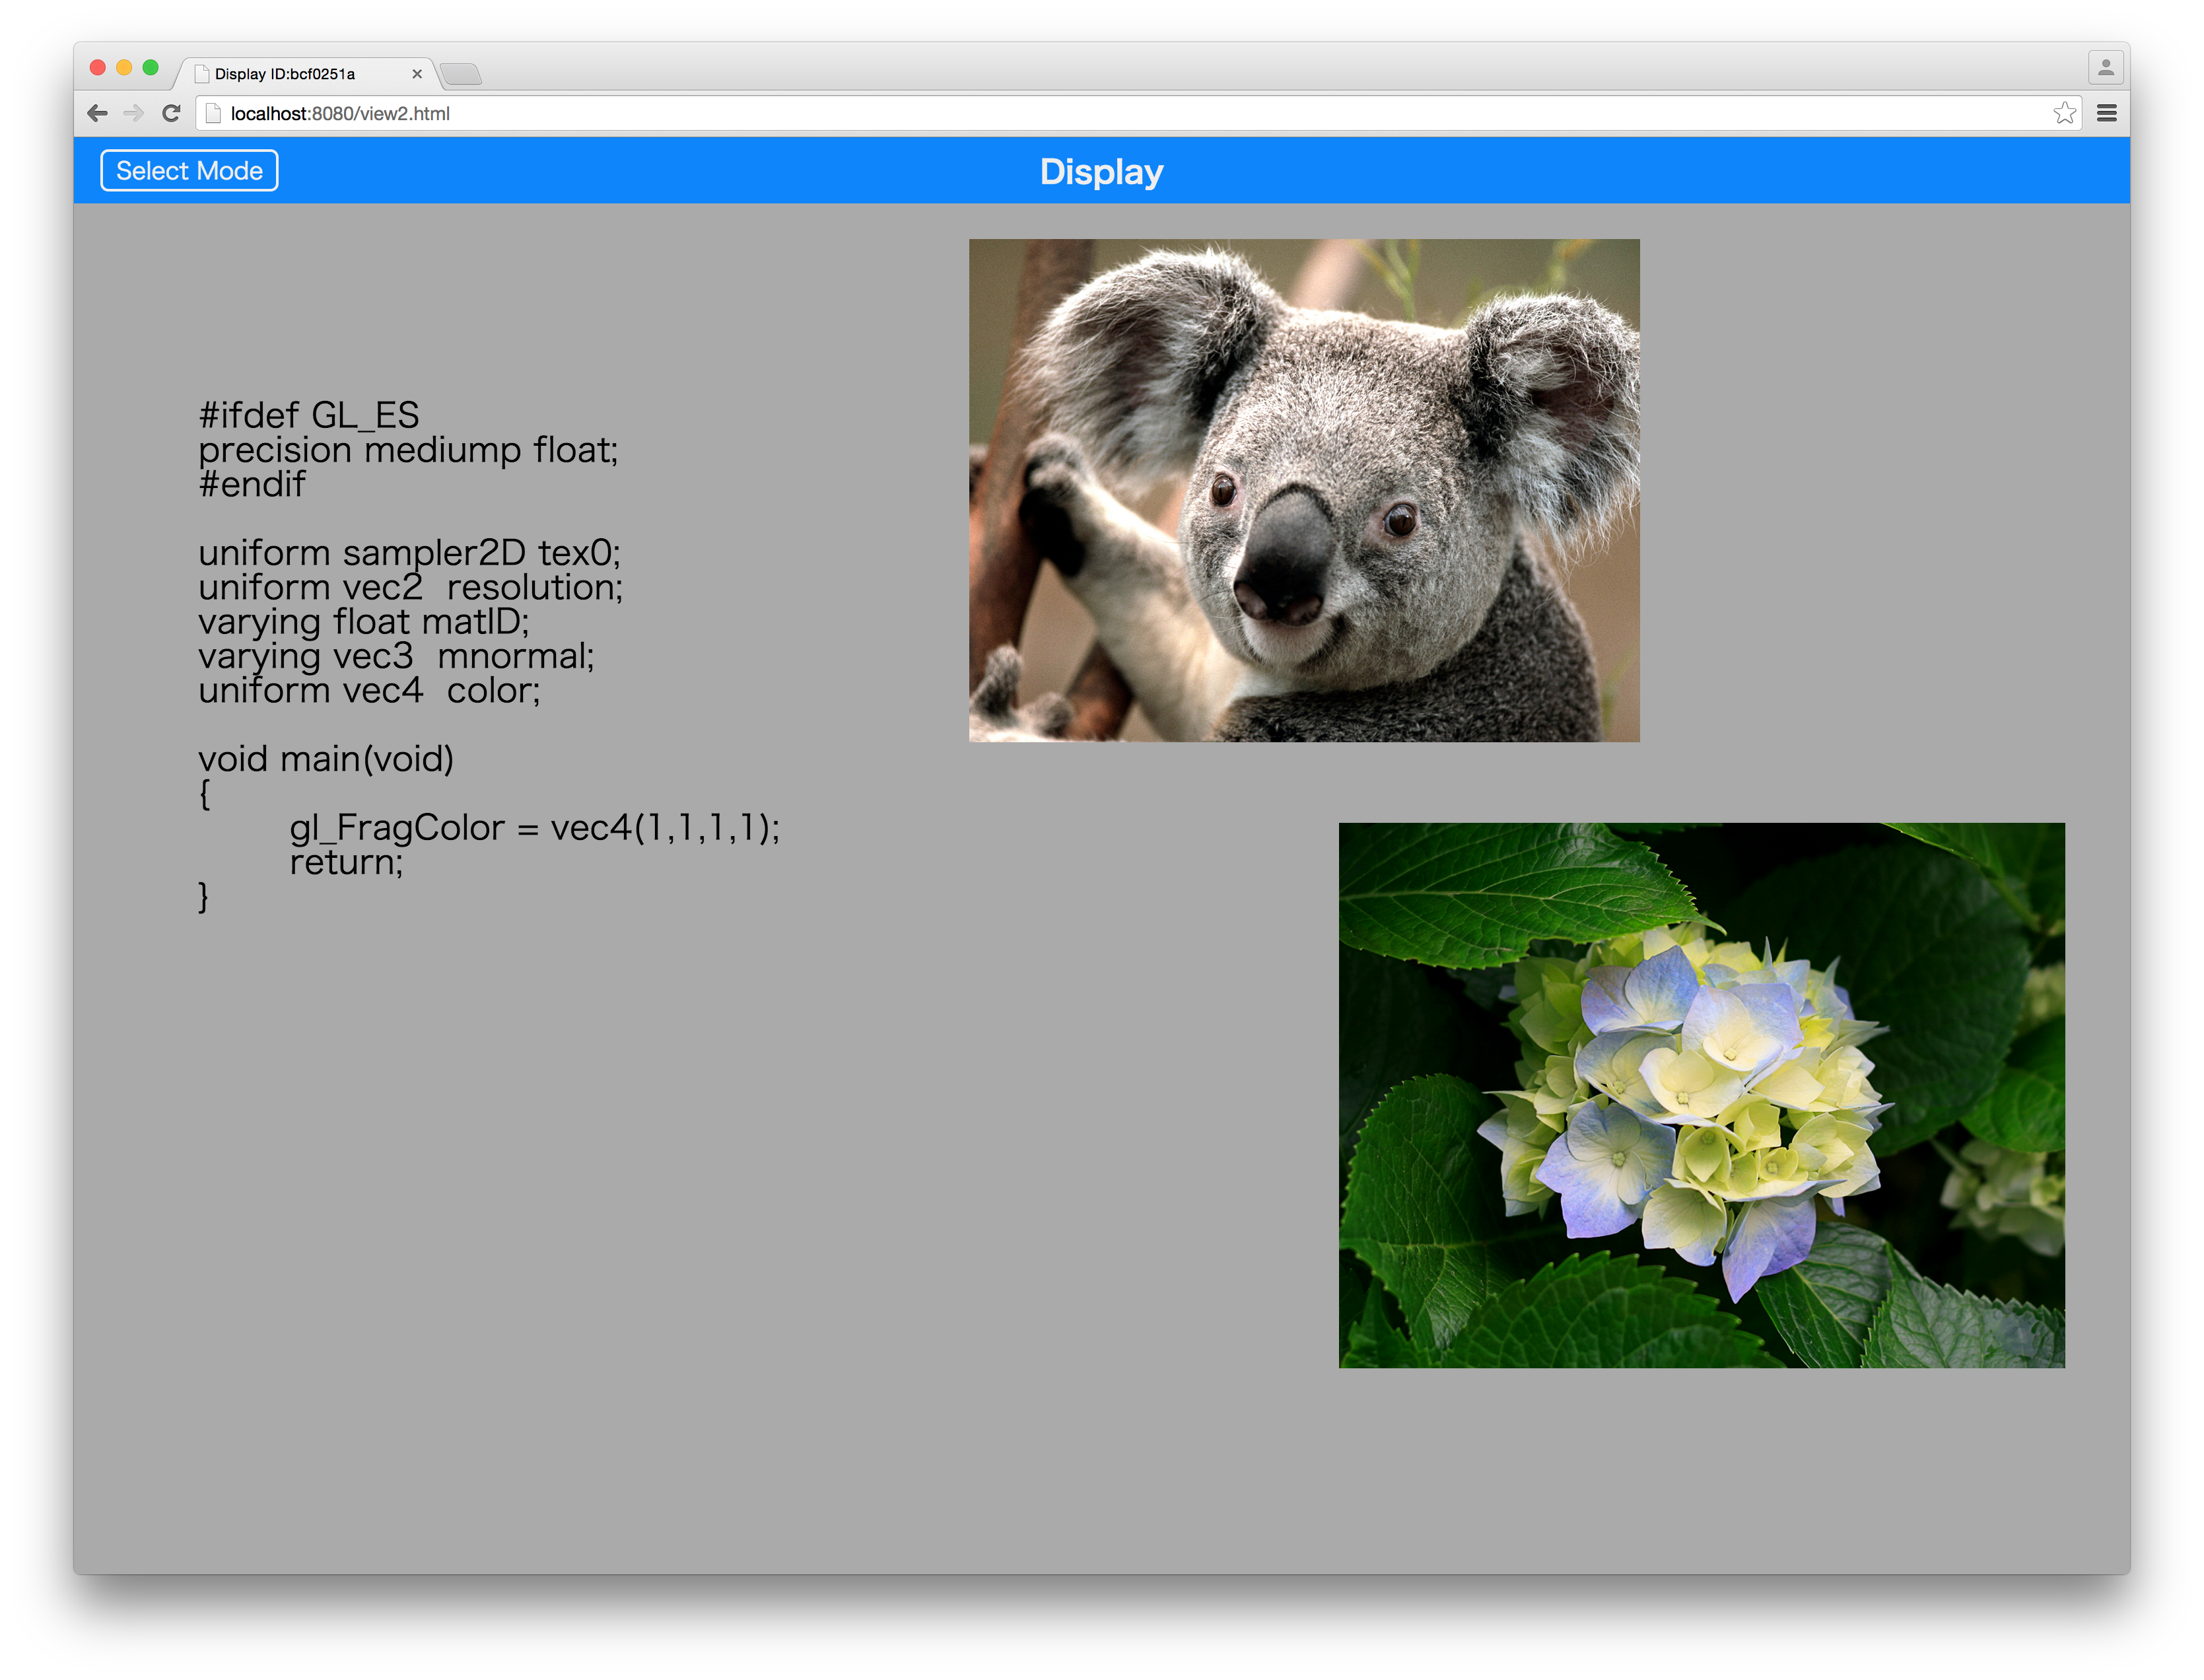
\includegraphics[width=14.5cm]{image/display.png}
	\end{center}
	\caption{ディスプレイ画面}
	\label{fig:display}
\end{figure}

\chapter{通信用APIの仕様}
\label{connectionapi}
クライアントサーバ間の通信についての仕様を記載する.

サーバではクライアントからwebsocketまたはsocekt.ioでメタバイナリを受け取り, メタデータに記載されているコマンドによって処理を行う. 処理を実行した後, クライアントに対して, レスポンスを含んだメタバイナリをwebsocketまたはsoceket.ioにて送信する.

データの更新が発生した際は, 更新通知をクライアントに対してブロードキャストする.
ディスプレイは, 更新通知を受け取ると, サーバへコンテンツ/ウィンドウ情報取得リクエストを送り, コンテンツ/ウィンドウ情報を取得する.

また, ディスプレイ新規表示時には, ディスプレイからサーバへ, ディスプレイ登録リクエストを発行し, 自身のディスプレイを登録する.

\begin{figure}[htbp]
	\begin{center}
		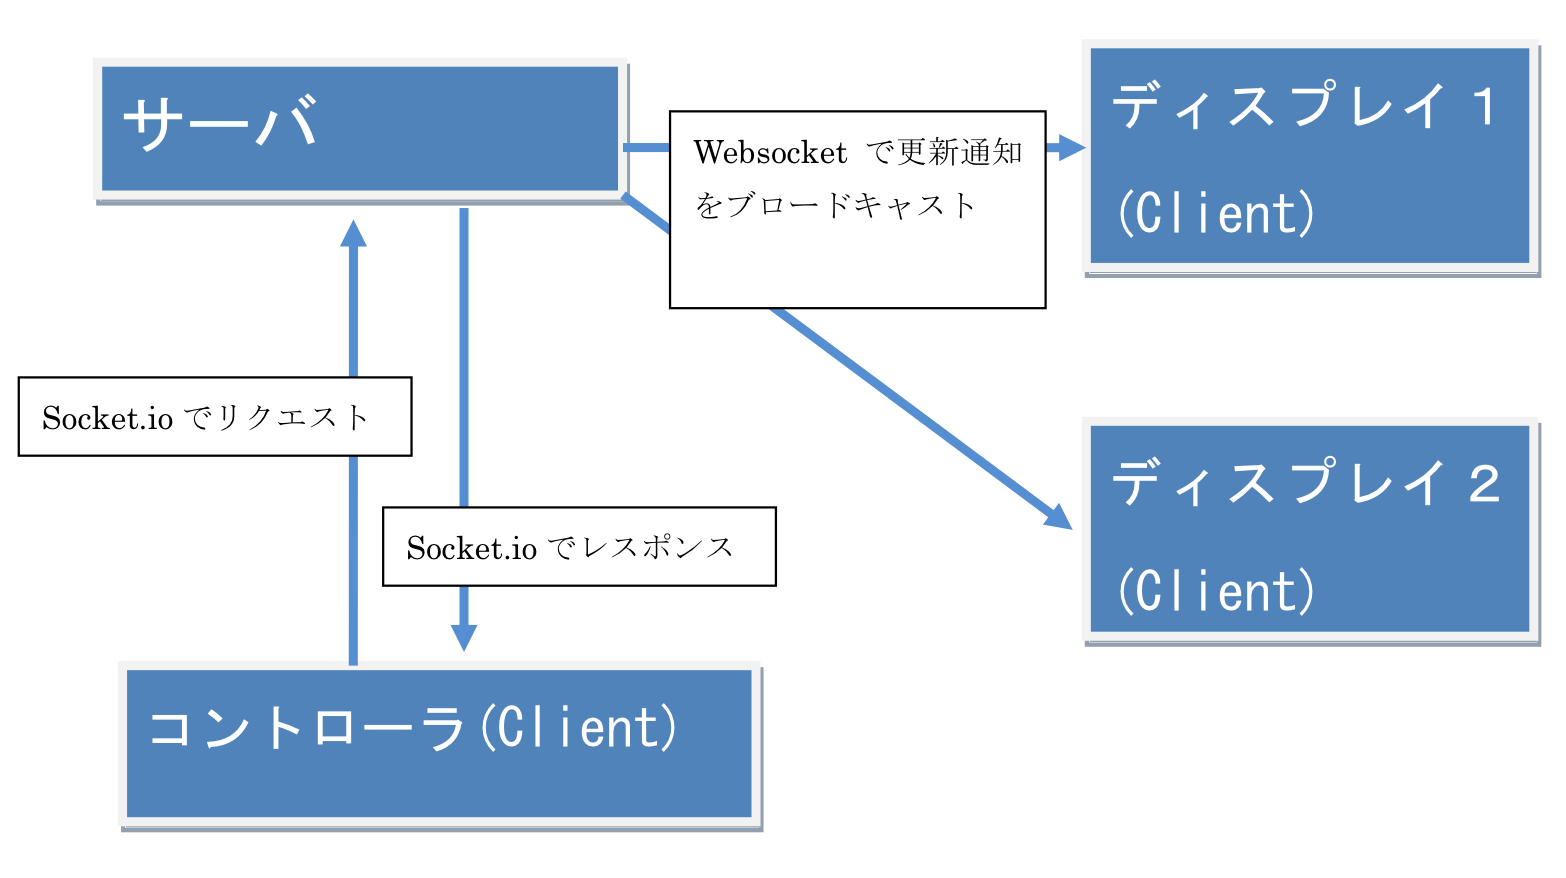
\includegraphics[width=14.5cm]{image/connection.png}
	\end{center}
	\caption{更新通知}
	\label{fig:connection}
\end{figure}

\newpage

\section{メタバイナリ}

クライアントサーバ間でやり取りするデータである, メタバイナリフォーマットのフォーマットを表\ref{metabin}に示す.


\begin{table}[htbp]
\begin{center}
\caption{メタバイナリフォーマット}
\label{metabin}
\begin{tabular}{|l|l|l|}
\hline
ヘッダ & "MetaBin:" (文字列) & 8 byte   \\
\hline
バージョン & UInt32 & 4 byte \\
\hline
メタデータサイズ & UInt32 & 4 byte \\
\hline
メタデータ & Ascii文字列(JSON) & メタデータサイズ \\
\hline
コンテンツデータ & Binaryなど & 残りの byte \\
\hline

\end{tabular}
\end{center}
\end{table}

コンテンツデータは, 具体的に以下の値が入る.
\begin{itemize}
\item メタデータの\verb+type = text+の場合:UTF8文字列
\item メタデータの\verb+type = url+の場合: URLエンコードされた文字列
\item メタデータの\verb+type = image+の場合: 画像ファイルのバイナリ
\end{itemize}

バージョンは, 現在常に1が入る.

\section{リクエスト/レスポンスコマンド}

サーバで受け付けているコマンドの一覧を, 表\ref{servercommands}に示す. 



\begin{table}[htbp]
\begin{center}
\caption{サーバーコマンド一覧}
\label{servercommands}
\begin{tabular}{|l|l|l|l|}
\hline
リクエストコマンド & レスポンスコマンド   &  実行内容   &   更新通知 \\
\hline
\hline
reqAddContent	& doneAddContent & コンテンツを追加します		& update \\
\hline
reqGetContent 	& doneGetContent & コンテンツを追加します		& 無し \\
\hline
reqGetMetaData & doneGetMetaData & メタデータを取得します		& 無し \\
\hline
reqDeleteContent & doneDeleteContent & 登録されているコンテンツを削除します		& update \\
\hline
reqUpdateContent & doneUpdateContent	& コンテンツを更新します		& updateTransform \\
\hline
reqUpdateTransform	& doneUpdateTransform & コンテンツのメタデータを更新します		& updateTransform \\
\hline
reqAddWindow	& doneAddWindow & ウィンドウを追加します		& updateWindow \\
\hline
reqDeleteWindow & doneDeleteWindow & ウィンドウを削除します		& update \\
\hline
reqGetWindow	& doneGetWindow & ウィンドウを取得します		& 無し \\
\hline
reqUpdateWindow & doneUpdateWindow	& ウィンドウのメタデータを更新します		& updateWindow \\
\hline
reqUpdateVirtualDisplay & doneUpdateVirtualDisplay & 仮想ディスプレイのメタデータを更新します		& updateWindow \\
\hline
reqGetVirtualDisplay	& doneGetVirtualDisplay & 仮想ディスプレイのメタデータを取得します	& 	無し \\
\hline
reqShowWindowID & doneShowWindowID & \shortstack[l]{ウィンドウIDを画面に表示するリクエスト \\ です. 全てのDisplayに更新通知 \\ showWindowIDが送信されます.}	& 	showWindowID \\
\hline

\end{tabular}
\end{center}
\end{table}


\newpage

\section{更新通知コマンド}

サーバから送信される更新通知コマンドの一覧を表\ref{responsecommands}に示す.

\begin{table}[htbp]
\begin{center}
\caption{更新通知コマンド一覧}
\label{responsecommands}
\begin{tabular}{|l|l|l|l|}
\hline
サーバからの更新通知コマンド	  & 通知内容 \\
\hline
\hline
update & \shortstack[l]{指定のIDまたは全てのコンテンツ/ウィンドウ \\ のデータが更新されたことを通知します.} \\
\hline
updateTransform & \shortstack[l]{指定のIDまたは全てのコンテンツ/ウィンドウ\\のメタデータが更新されたことを通知します.} \\
\hline
updateWindow & \shortstack[l]{指定のIDまたは全てのウィンドウが、\\ 追加または更新されたことを通知します.} \\
\hline
showWindowID & ウィンドウIDを表示する必要があることを通知します。\\
\hline

\end{tabular}
\end{center}
\end{table}

\newpage

\section{コマンド送信例}
\subsection{画像登録の例}

登録するコマンドと, 幅や高さなどの情報を, メタデータとしてJSON形式で定義する.

\begin{verbatim}
metadata = {
    "command": "reqAddContent", 
    "type": "image", 
    "posx": 100, 
    "posy": 200, 
    "width": 500,
    "height": 400 
};
\end{verbatim}

\verb+metadata+と, 画像などのバイナリデータを組み合わせて,メタバイナリを作成する. 

\begin{table}[htbp]
\begin{center}
\caption{送信するメタバイナリ}
\label{sendmetabin}
\begin{tabular}{|l|l|l|l|l|}
\hline
"MetaBin:" & \verb+1+ & \verb+metadata+のサイズ & \verb+metadata+ & バイナリデータ \\
\hline

\end{tabular}
\end{center}
\end{table}

コントローラから, サーバに, メタバイナリを送信することで, 画像が登録される. サーバでは登録時に,
オリジナルのイメージサイズを, \verb+orgWidth+, \verb+orgHeight+ としてメタデータに追加する. 
登録が終了したら, “doneAddContent”コマンドを含んだ, メタデータがコントローラに返信される. 

返信されるメタデータ

\begin{verbatim}
Metadata = {
    "command": "doneAddContent", 
    "id": "8ba1dwm", 
    "type": "image", 
    "posx": 100, 
    "posy": 200, 
    "width": 500,
    "height": 400 ,
    “orgWidth”: 500,
    “orgHeight” : 400
};
\end{verbatim}


\chapter{データ構造について}
\label{redisdb}

\section{DBのデータ構造}

本システムは, データベースとしてredisを使用しており, サーバによって受け付けたコンテンツやウィンドウ情報を保存している. 表\ref{dbstructure}に, DBのデータ構造を示す.
\begin{table}[htbp]
\begin{center}
\caption{DBのデータ構造}
\label{dbstructure}
\begin{tabular}{|l|l|l|l|}
\hline
キー	& 内容 & 意味 \\
\hline
\hline
tiled\_server:s:default:virtual\_display & splitX & 仮想ディスプレイ全体のx方向分割数 \\
 	& splitY	 &仮想ディスプレイ全体のy方向分割数 \\
 	& orgWidth & 仮想ディスプレイ全体の幅 \\
 	& orgHeight & 仮想ディスプレイ全体の高さ \\
\hline
tiled\_server:s:default:content:[コンテンツID] & \shortstack[l]{バイナリまたは\\テキストデータ}	& コンテンツの実データ \\
\hline
tiled\_server:s:default:metadata:[コンテンツID] & id & コンテンツID \\
 	& type & コンテンツの種類 \\
 	& posx & x座標 \\
 	& posy & y座標 \\
 	& width & 幅 \\
 	& height & 高さ \\
 	& orgWidth &初期幅 \\
 	& orgHeight & 初期高さ \\
 	& zIndex & zインデックス \\
 	& visible & 表示状態 \\
 	& mime & 	mimeタイプ \\
\hline
tiled\_server:s:default:window:[ウィンドウID] & id & ウィンドウID \\
 	& type & window \\
 	& posx &  x座標 \\
 	& posy & 	y座標 \\
 	& posx & 	x座標 \\
 	& posy & 	y座標 \\
 	& width & 	幅 \\
 	& height & 	高さ \\
 	& orgWidth & 	初期幅 \\
 	& orgHeight & 	初期高さ \\
 	& visible & 	表示状態 \\
\hline
tiled\_server:s:tiled\_server:sessions & default & セッションID \\
\hline

\end{tabular}
\end{center}
\end{table}


\section{データ格納方法について}
\subsection{IDについて}
コンテンツ情報, ウィンドウ情報は, それぞれコンテンツID, ウィンドウIDを割り当てて, データを格納している. IDはサーバでコンテンツ保存時に, ランダムな英数字8桁で作成される, “reqAddContent”などの追加コマンドに, 任意のIDを指定して追加することができる.

\subsection{格納形式について}
画像データ, テキストデータは, クライアントから送信されたものをそのままバイナリまたはUTF8文字列として保存している. URLについては, phantom.jsでレンダリングした画像データをバイナリとして保存している.

\subsection{サーバで付与するメタデータについて}
画像データについては, サーバ側で保存する際に, mimeを自動判別して保存している. また, phantomjsでレンダリングした画像については, \verb+posx+, \verb+posy+, \verb+width+, \verb+height+, \verb+orgWidth+, \verb+orgHeight+ を, サーバ側で付与している.


\chapter{コントローラについて}
コントローラページでは, コンテンツとディスプレイに対して各種操作を行うページである. 具体的には, コンテンツの登録, 削除, 移動, 拡大縮小, ディスプレイの削除, 移動, 拡大縮小, 仮想ディスプレイ全体の大きさの更新, 仮想ディスプレイ分割数の変更を行うことができる.

\section{コンテンツの登録について}
コントローラにて, 画像ファイル, テキスト, テキストファイル, URLをコンテンツとして登録することができる. 画像ファイルはjpg, gif, png, bmp形式に対応している. また, URLはサーバにてpng形式の画像としてレンダリングされて登録される.


\begin{table}[htbp]
\begin{center}
\caption{コンテンツの種類}
\label{contentstype}
\begin{tabular}{|l|l|l|}
\hline
コンテンツの種類 & 形式 & 備考 \\
\hline
\hline
テキスト & 文字列 & \\
\hline
テキストファイル & txt & \\
\hline
画像	& jpg, gif, png, bmp & \\
\hline
URL	& png & サーバサイドレンダリング \\
\hline

\end{tabular}
\end{center}
\end{table}

\section{仮想ディスプレイ全体の設定について}
仮想ディスプレイ全体の設定として, 仮想ディスプレイ全体の幅, 高さ, 分割数を設定することができる. 

\section{コンテンツ/ディスプレイの設定について}
登録したコンテンツ及びディスプレイは, 仮想ディスプレイを表す矩形上に, 自由に配置し,移動, 拡大縮小等を行うことができる. また, スナップ設定を有効にすることで, 仮想ディスプレイの分割領域に対してフィットするように配置することができる.

\subsection{コンテンツ設定}
コンテンツは, x(x座標), y(y座標), w(幅), h(高さ), z(zIndex)のプロパティを持っており, 移動, 拡大縮小,zオーダーの変更を行うことが出来る.

\subsection{ディスプレイ設定}
ディスプレイは, w(幅), h(高さ), split x(x方向分割数), spilt y(y方向分割数)のプロパティを持っており, w, hを変更することで, 幅, 高さの変更を行うことが出来る. 
また, split x, split y を変更することで, 各方向に指定した分割数で仮想ディスプレイが分割される.

\subsection{スナップについて}
スナップ設定は, Free または Display から選択でき, Freeを選択した場合はスナップ設定が無効になり Displayを選択した場合はスナップ設定が有効になる.
スナップ設定が有効の場合, コンテンツでもディスプレイでも同様に, 仮想ディスプレイの分割領域に対してフィットするように配置することができる.
配置した際は, 左上が原点となり, 分割領域に収まるようにコンテンツまたはディスプレイが, アスペクト比を保った状態でリサイズされる.\\

分割した領域に対してスナップ配置しているイメージを図\ref{fig:fitbefore}, 図\ref{fig:fitafter}に示す. 


\begin{figure}[htbp]
	\begin{center}
		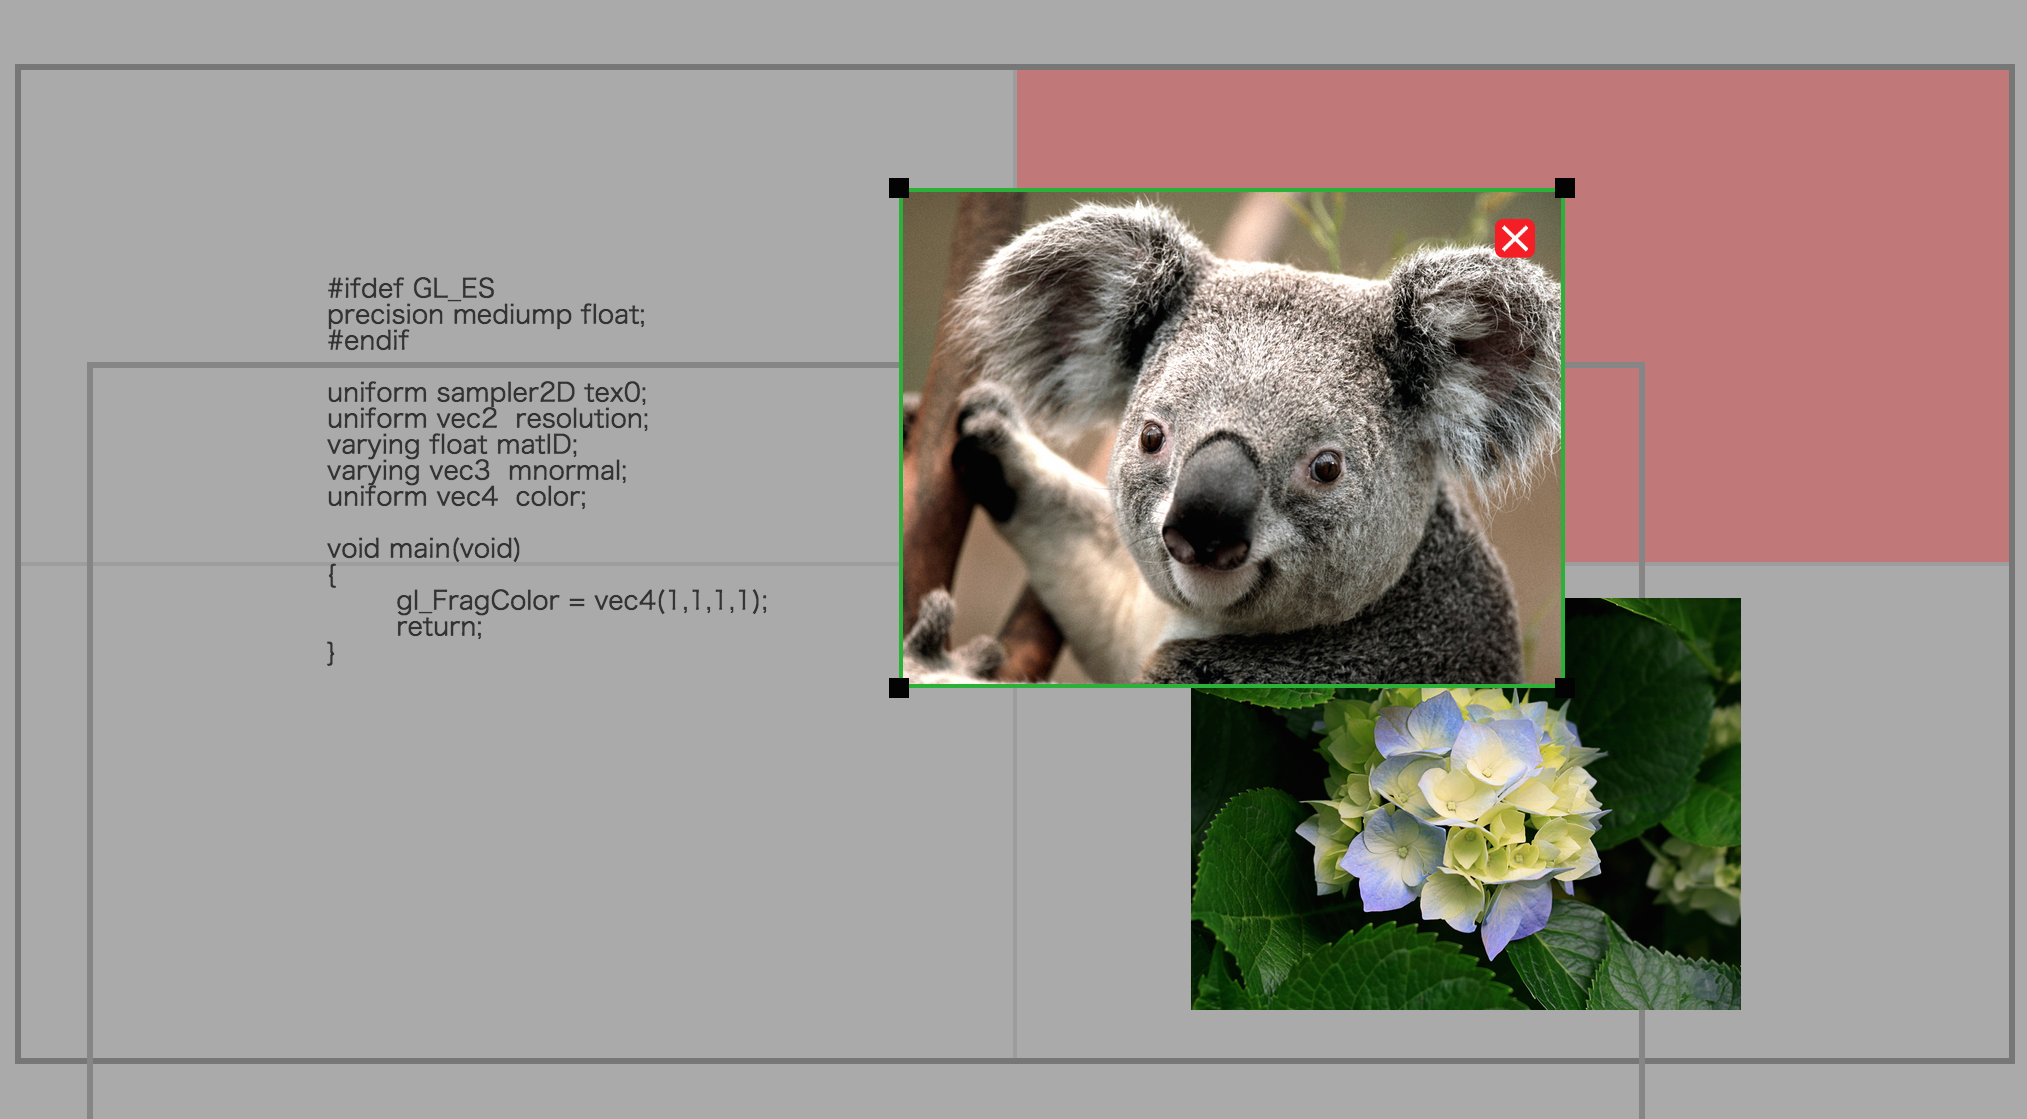
\includegraphics[width=11.5cm]{image/fitbefore.png}
	\end{center}
	\caption{スナップ配置前}
	\label{fig:fitbefore}
\end{figure}

\begin{figure}[htbp]
	\begin{center}
		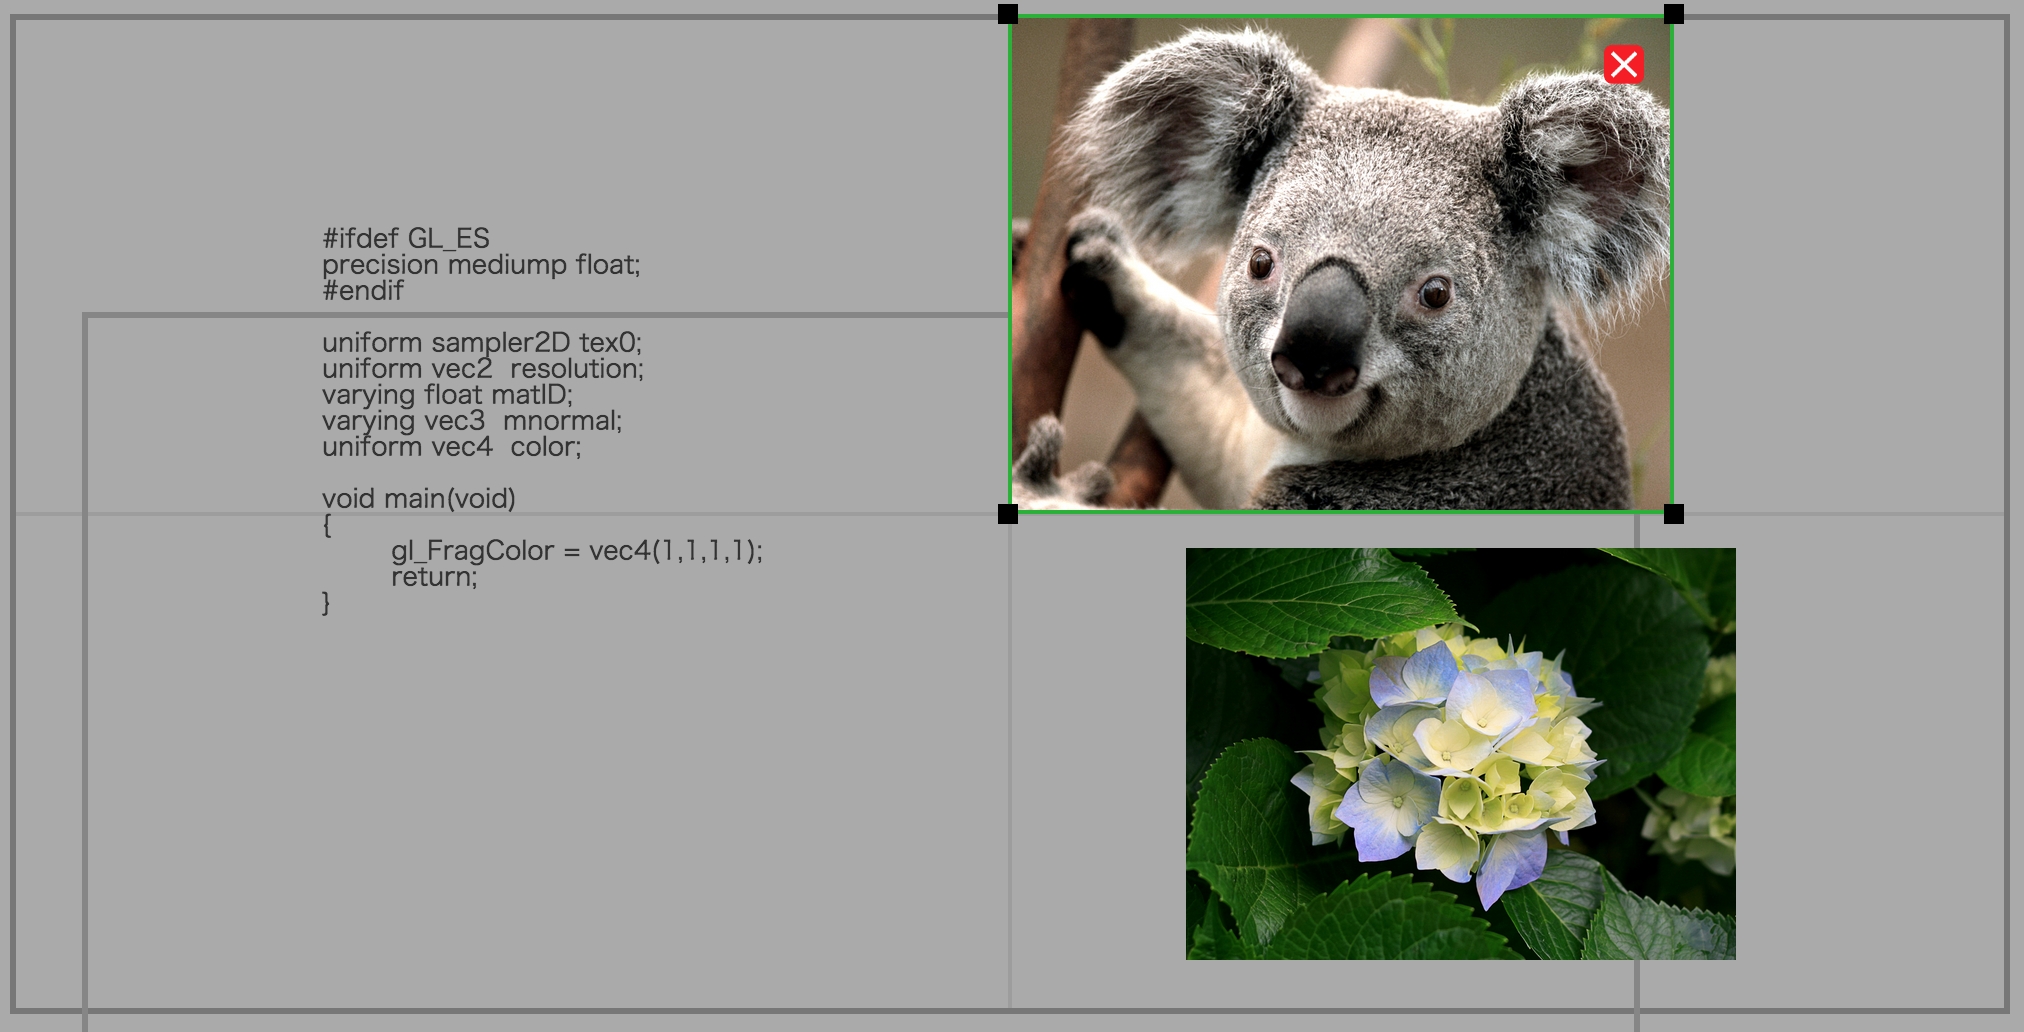
\includegraphics[width=11.5cm]{image/fitafter.png}
	\end{center}
	\caption{スナップ配置後}
	\label{fig:fitafter}
\end{figure}

\chapter{ディスプレイについて}
ディスプレイページでは, コントローラで操作した結果のコンテンツを表示することができるページである. 操作は全てコントローラより行う仕様となっている.

\section{ディスプレイの登録について}
サーバが起動した状態でディスプレイページを開くと, websocketのAPIを用いて自動的にサーバに登録される. 登録後は, コントローラにてコンテンツと同様に配置, 移動することができ, ディスプレイページを閉じると自動的に登録が解除される. 

\chapter{動作環境について}
Windows, Linux, MacOSXのGoogleChrome, Firefox及びSafariで動作する.
各ブラウザの最新のバージョンにて動作確認を行う.

\subsection*{動作確認環境}
\begin{itemize}
	\item IA-32/Intel64上で動作するLinux
	\begin{tabbing}
		1234\=123456789012\=012345678901234567890\kill
		\> OS \> : CentOS Linux 6.6 x64 \\ 
		\> Webブラウザ \> : Firefox 33.0
	\end{tabbing}
	\item IA-32/Intel64上で動作するWindows
	\begin{tabbing}
		1234\=123456789012\=012345678901234567890\kill
		\> OS \> : Windows7 64bit \\
		\> Webブラウザ \> : Firefox 33.0, Chrome 41, Internet Explorer 11
	\end{tabbing}
	\item IA-32/Intel64上で動作するMac OS X
	\begin{tabbing}
		1234\=123456789012\=012345678901234567890\kill
		\> OS \> : Mac OS X 10.10(Yosemite)\\
		\> Webブラウザ \> : Firefox 33.0, Chrome 41, Safari 7.1.4
	\end{tabbing}
\end{itemize}

\chapter{モジュール構成}
\section{サーバサイド}
\begin{itemize}
\item server/server.js  - Websocket/Socket.io/HTTPのサーバ
\item server/operator.js - DBへの読み書き, socket.io/websocketの全コマンドの処理を記述している.
\item server/sender.js - websocketによるビュー用のコマンド送受信処理を記述している. 内部的にはoperator.jsのインスタンスを使用して処理している.
\item server/util.js - ファイル入出力などのユーティティ
\item server/metabinary.js - メタバイナリを作成するための処理
\item server/command.js - 全てのコマンド名を定義している
\item server/capture.js - phantom.js でURLをレンダリングするための処理を記述している
\end{itemize}

\section{クライアントサイド}
\begin{itemize}
\item client/js/controller2.js - コントローラの内部処理
\item client/js/view2.js - ディスプレイの内部処理
\item client/js/vscreen.js - 仮想スクリーン(全体, 個別)の矩形の処理をまとめたクラス
\item client/js/vscreen\_util.js - 仮想スクリーンの矩形処理とmetadataに関するユーティリティ
\item client/js/animtab.js - タブのアニメーションモジュール
\item client/js/manipulator.js - コンテンツ/ウィンドウのマニピュレータの表示,削除,移動処理
\item client/js/index.html - トップページ
\item client/js/controller2.html - コントローラページ
\item client/js/view2.html - ディスプレイページ
\end{itemize}

\end{document}




